\chapter{仿真实验与结果分析}
在第三章中我们设计实现了多跳长路径上多节点联合数据认证机制,第三章中提出了对多节点联合数据机制的优化方案,并对它们进行了理论分析。在本章中我们将使用仿真实验平台,对数据认证机制进行实验验证,并对它们的性能进行比较分析。6.1节介绍实验平台的环境,及相关仿真软件的介绍。6.2节是多跳长路径上多节点联合数据认证仿真实验及结果分析。6.3节是数据认证优化方案仿真实验及结果分析。
\section{实验平台环境}
\subsection{仿真实验环境}
为了搭建无线传感网的仿真环境,本文采用了仿真平台OMNeT++(Objective Modular Network testbed in C++)进行仿真,在Windows 7 的主机中安装的版本为OMNeT++4.6b1。 主机的配置为:
\begin{compactitem}
  \item DDR3内存,容量8G,频率1600MHz
  \item Core 双核处理器,主频2.6GHz
\end{compactitem}

现在进行网络仿真的工具很多,还有有NS2、NS3、OPNET、TOSSIM、GloMoSim和PowerTOSSIM等平台。NS2和NS3平台虽然有丰富的协议库支持,但是仿真时数据量过大,对复杂的无线传感网场景的仿真不合适,而且学习曲线比较高。OPNET平台要实现无线传感网仿真,学习门槛较高,而且其最大问题是提供的类库太少,仿真速度慢。TOSSIM、GloMoSim和PowerTOSSIM等其他仿真平台也有相应的局限性。

本文的实验中,我们选择了OMNeT++ 平台,OMNeT++是面向对象的离散事件仿真工具。OMNeT++基于Eclipse平台构建,是一款开源的仿真集成环境,由建模工具、仿真运行工具和输出结果分析工具等组成。OMNeT++还有INET、INETMANET或MIXIM等类库支持网络仿真,利用这些开源的包,很容易对各种网络协议进行仿真实验。

在OMNeT++中,主要使用C++语言创建仿真对象类,并使用ned文件配置仿真的参数,一个OMNeT++的仿真模型包括如下部分:
\begin{enumerate}\setlength{\itemsep}{-\itemsep}
  \item 网络拓扑结构描述文件(.ned文件):使用ned文件对仿真网络中的信道、门、连接和模块等进行配置。
  \item 消息或包定义文件(.msg文件):对网络中传输的消息或者数据报文进行定义,OMNeT++会自动从.msg生成相应的消息类。
  \item 模块描述文件(.h和.cc文件):使用C++语言描述模型中的各个模块。
\end{enumerate}
仿真模型使用C++编译器将.ned网络拓扑结构描述文件、.msg消息或包定义文件以及模块描述文件进行编译后,同仿真内核库以及用户接口库进行链接,生成可执行的仿真程序。OMNeT++不同于其他仿真平台,生成的仿真程序可以运行于没有安装OMNeT++的机器上。

\subsection{数据认证仿真框架}
下面将对搭建的无线传感网数据认证仿真模型进行介绍,
在我们的无线传感网数据认证机制研究中,我们的仿真模型主要包括两种对象:传感器节点和基站。
在本文中,我们假设所有的传感器节点均为相同的配置,部署时的能量相同。

\subsubsection{模块配置}
在OMNeT++仿真平台中,使用ned文件配置相应的模块,
传感器节点的配置文件如下所示,节点包括了一个输入输出门向量:
\begin{lstlisting}[language=C]
simple Node
{
    parameters:
        double txRate @unit(bps);
        double radioDelay @unit(s);       // 时间片
        volatile double iaTime @unit(s);  // 数据包发送间隔时间
        @display("i=device/wsn");
    gates:
        inout out;
}
\end{lstlisting}
基站的配置文件如下所示,基站也包括一个输入输出门向量,仿真实验中假设基站的通信不会受信道冲突的影响:
\begin{lstlisting}[language=C]
simple Bs
{
    parameters:
        @display("i=device/antennatower_l");
    gates:
        inout bsRadio[];
}
\end{lstlisting}
\subsubsection{模块类实现}
在我们的仿真实验中,传感器节点模块和基站模块都使用C++编写,我们对两个模块的实现做简要的介绍。

传感器节点使用了固定时间间隔内随机生成数据报文的方式仿真数据采集的过程,并采用自消息完成数据传输给簇头的过程,其采集过程函数表示如下:
\begin{lstlisting}[language=C]
void Node::initialize() {
    char msgname[20];
    sprintf(msgname, "event sensor # %d", getIndex());
    startEvent = new cMessage(msgname);
    iaTime = &par("iaTime");
    radioDelay = par("radioDelay");
    //事件捕获后的发送时间
    simtime_t t = simTime() + iaTime->doubleValue();
    if (ev.isGUI())
        getDisplayString().setTagArg("t", 2, "#808000");
    scheduleAt(t, startEvent);
}
\end{lstlisting}

传感器节点仿真发送数据包的过程主要由函数handleMessage完成:
\begin{lstlisting}[language=C]
void Node::handleMessage(cMessage* msg) {
    int src = getIndex();
    char msgname[40];
    sprintf(msgname, "event from cluster node %d", src);
    PacketCn *pkt = new PacketCn(msgname);
    pkt->setBitLength(952);
    pkt->setSource(src);
    pkt->setEvent(event);
    WATCH(pkt);
    //下一个事件发送时间,形成一个包传送给BS
    simtime_t tt = simTime() + iaTime->doubleValue();
    simtime_t nextTime=0;
    if((ceil(simTime()/radioDelay)*radioDelay)<tt)
        nextTime = tt;
    else
        nextTime = tt+radioDelay;
    ev << "send packet:"<<pkt<<" when "<<nextTime<< endl;
    send(pkt, "out$o");
    scheduleAt(nextTime, startEvent);
}
\end{lstlisting}

基站模块主要是接收数据报文,并对报文中的XMAC进行认证,确定报文的身份,其主要函数如下:
\begin{lstlisting}[language=C]
void Bs::handleMessage(cMessage* msg) {
    PacketCh *pkt = check_and_cast<PacketCh *>(msg);
    int event=pkt->getEvent();
    //计算event的XMAC
    int eventMac=this->Xmac(event);
    if(pkt->getXmac()==eventMac){
        ev<<"event received!"<<endl;
    }
    else{
        ev<<"trash packet!"<<endl;
    }
    delete pkt;
}
\end{lstlisting}

\section{仿真实验与方案评估}
在本节中我们对第三章和第四章中提出的数据认证方案进行仿真实验,并对它们的安全性能和能量开销进行分析评价。

我们的仿真条件是将1000个无线传感器节点部署到$150\times 100 m^2$大小的平面监测区域中,使用OMNeT++中的协议栈开源包在无线传感网中完成建簇过程,每个节点簇大小为$10 \times 10 m^2$,并完成传输路径的建立。每个传感器节点具有相同的硬件配置和通信能力,且每个节点的初始化能量为$1J$。在节点间的单跳通信中,发送1 字节报文需要$16.25 \mu J$能量,接收1字节报文需要$12.5 \mu J$ 能量,报文的大小为$24 byte$,报文中的每个MAC大小为$1 byte$。在每个节点进行认证时,计算一个MAC 需要的能量为$15 \mu J$。


\subsection{多跳长路径上多节点联合数据认证仿真实验}
在对多跳长路径上多节点联合数据认证机制(Multi Node Authentication,简称MNA方案)的仿真实验中,基站能够在初始化阶段通过每个部署节点的位置信息以及分配的ID建立多跳长路径。在各个簇与基站之间的路径上,通过HELLO报文和ACK报文完成上下行相关节点的发现,节点保存上下行相关节点的ID信息并建立共享密钥。

在实验中,每个簇内节点在一定的时间片内随机产生一个采集信息消息发送给簇头节点,当簇头节点收集到一定数量的采集信息消息以后进行数据聚合并发送数据报文给基站,当整个传感网中产生1000个数据报文时,实验结束,实验流程如图~\ref{fig:MPAtest}所示:
\begin{figure}[htbp]
  \centering
  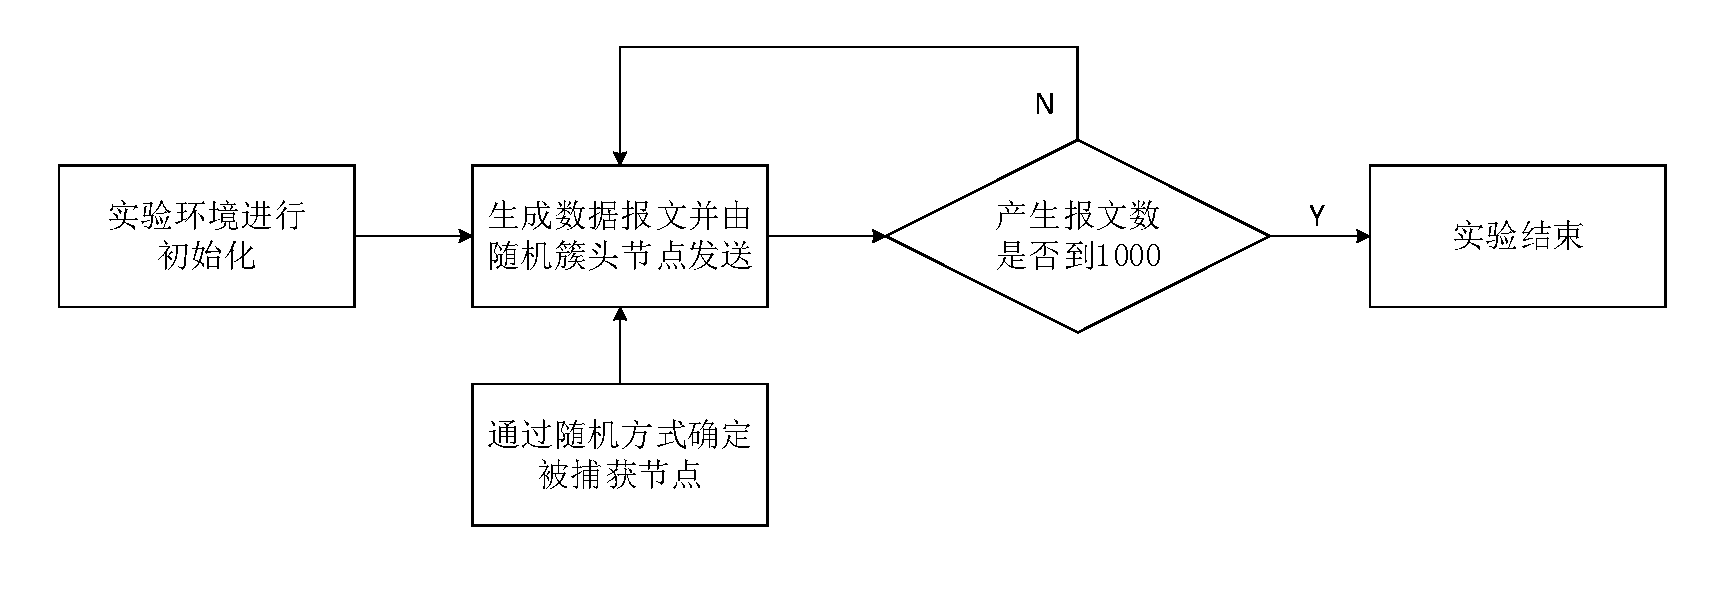
\includegraphics[width=6in]{MPAtest}
  \caption{多跳长路径上多节点联合数据认证仿真实验}
  \label{fig:MPAtest}
\end{figure}

每个节点都有一定的概率$p$被攻击而成为妥协节点,产生的1000个数据报文中既包括合法报文,也包括非法报文。网络中产生的非法数据报文的比例(Fabricated Reports Rate,简称FRR)是实验中被控制的变量,在不同的FRR下,我们进行仿真实验,并对结果进行分析。

如图~\ref{fig:MNAfilter}所示,是多跳长路径上多节点联合数据认证机制在参数$t=3$和$t=7$时路径中过滤比例同FRR的关系。横坐标是非法数据报文的比例FRR,纵坐标是路径中被丢弃的报文的比例。
仿真实验的结果表明我们的多跳长路径上多节点联合数据认证机制对虚假数据报文有较高的检测性能,大部分的虚假数据报文在路径中过滤阶段被丢弃。
由于仿真实验中,每个节点都有一定的概率$p$被攻击,因此路径中传输的虚假数据报文有可能因为攻击者利用多个被攻击节点合谋而绕过数据认证机制,最终被传输到基站。
可以看到在参数$t=3$,也就是簇规模较小时,相对$t=7$有更高的检测效率,我们的多节点联合数据认证机制在簇规模较小的无线传感网中有更好的安全性能。
\begin{figure}[htbp]
  \centering
  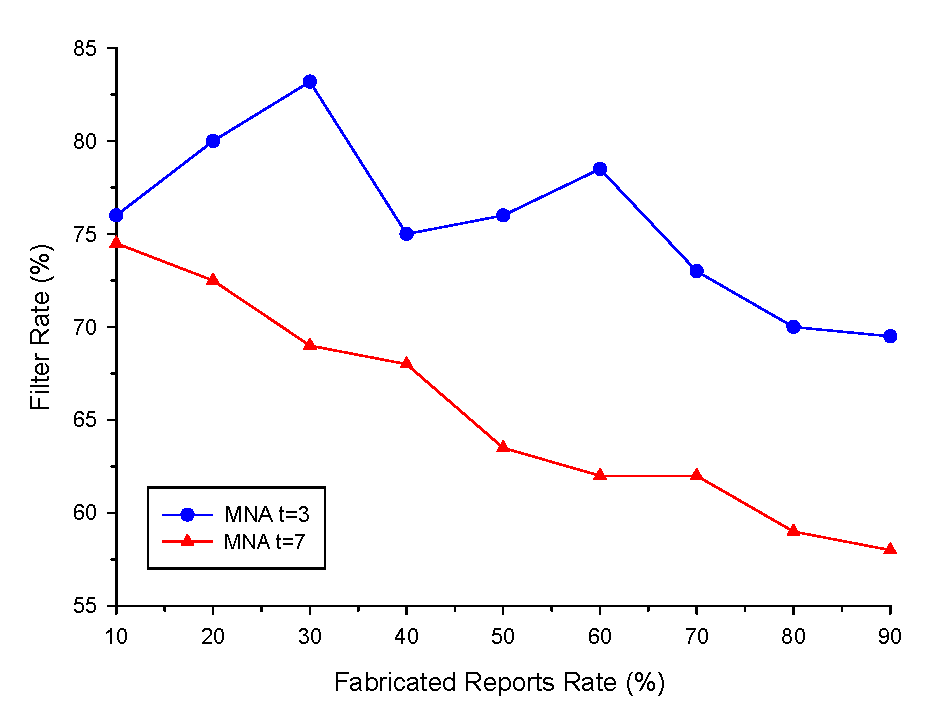
\includegraphics[width=5in]{MNAfilter}
  \caption{多节点联合认证的安全性能}
  \label{fig:MNAfilter}
\end{figure}

如图~\ref{fig:MNAenergy}所示,是多跳长路径上多节点联合数据认证机制在参数$t=3$和$t=7$时的能量开销,纵坐标是无线传感网中的总能量开销。可以从图中看出,能量开销随FRR的变大,基本是线性变化,因为当FRR变大时,有更多的报文在路径检测过程中被丢弃,减小了整个无线传感网中发送接收数据报文以及进行MAC计算完成认证的能量开销。在FRR较低时,簇规模对能量开销的影响不大,但是随着FRR的变大,簇规模较小的传感网比簇规模较大的传感网有更少的能量开销。

\begin{figure}[htbp]
  \centering
  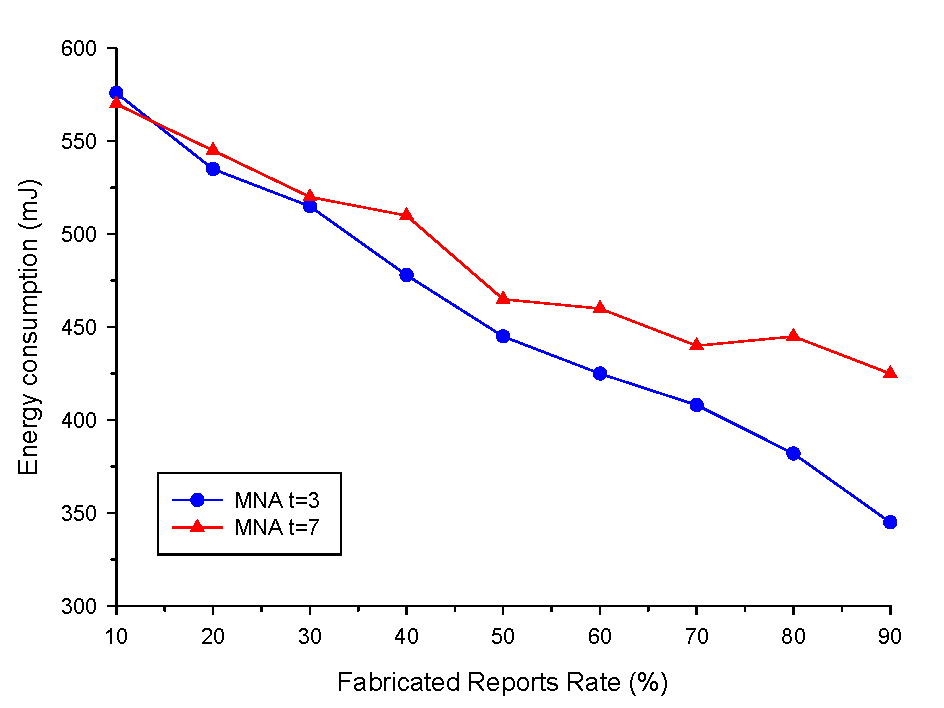
\includegraphics[width=5in]{MNAenergy}
  \caption{多节点联合认证的能量开销}
  \label{fig:MNAenergy}
\end{figure}

\subsection{数据认证优化方案仿真实验}
在对第四章提出的数据认证优化方案进行仿真实验时,实验条件与多跳长路径上多节点联合数据认证仿真实验相同。
\subsubsection{多路径抗节点失效机制的仿真实验}
为了增强数据认证机制的稳定性,在节点被攻击时保证数据认证机制的有效性,我们在4.1节提出了多路径抗节点失效的认证机制
(Multi Path Authentication,简称MPA)。

在初始化和密钥分配阶段,建立传输路径并完成上下行相关关系发现。在仿真实验中,利用相关机制建立两条备用不相交路径,以及两条编织路径。在实验中,每个簇内节点在一定的时间片内随机产生一个采集信息消息发送给簇头节点,当簇头节点收集到一定数量的采集信息消息以后进行数据聚合并发送数据报文给基站,当整个传感网中产生1000个数据报文时,实验结束。在对多路径抗节点失效机制进行仿真实验时,我们的无线传感网簇规模固定为$t=3$。

如图~\ref{fig:MPAfilter}所示,是多路径抗节点失效机制的路径中过滤比例同FRR的关系。在路径中检测率上,MPA方案相比MNA方案有较大的提升,而且MPA方案有更好的稳定性,在FRR变化时,MPA方案有比较稳定的检测率。
\begin{figure}[htbp]
  \centering
  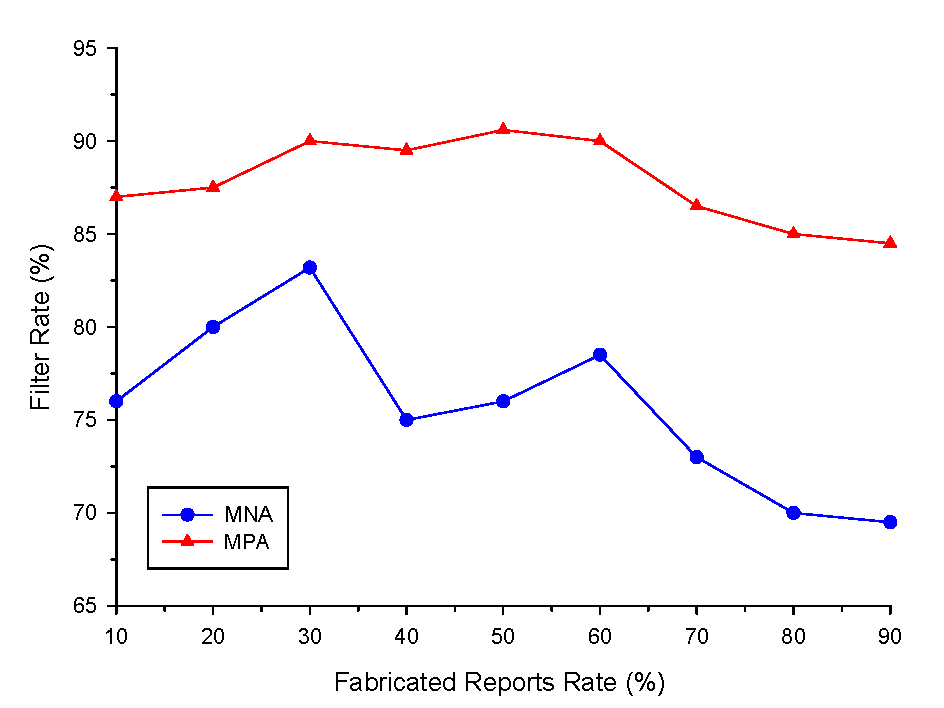
\includegraphics[width=5in]{MPAfilter}
  \caption{多路径抗节点失效机制的安全性能}
  \label{fig:MPAfilter}
\end{figure}

如图~\ref{fig:MPAenergy}所示,是多路径抗节点失效机制的能量开销。MPA方案和MNA方案的能量开销比较相近,在FRR较小时,由于MPA方案需要维护多条备用路径和编织路径,而且需要额外的hash函数运算,有更高的能量开销。随着FRR的变大,由于路径中检测率相比MNA 方案更高,虚假数据报文能更快的被丢弃,MPA方案的能量开销开始优于MNA方案。
\begin{figure}[htbp]
  \centering
  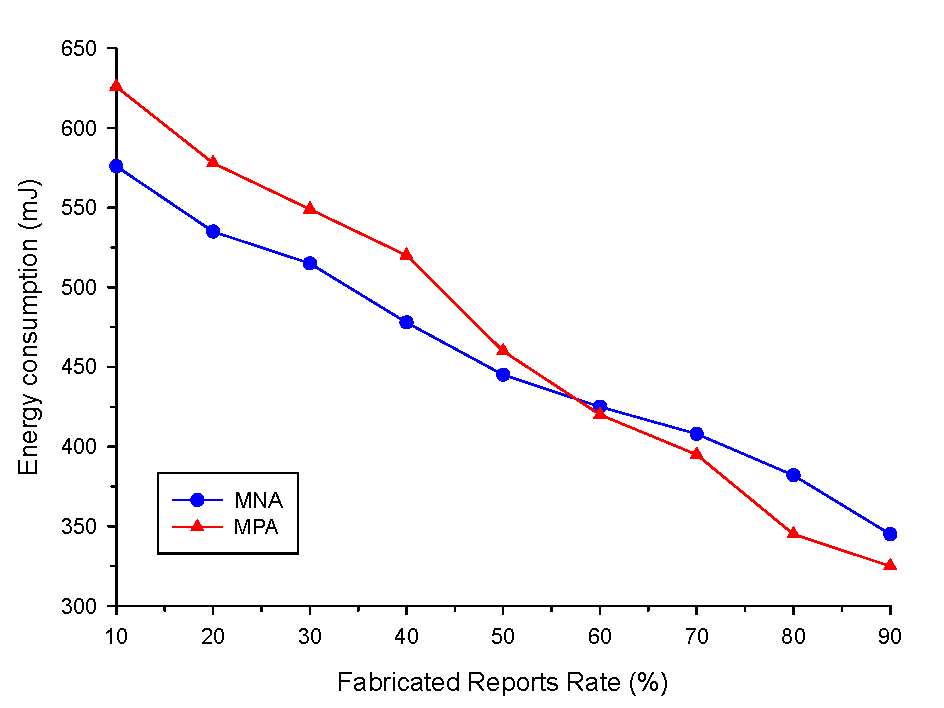
\includegraphics[width=5in]{MPAenergy}
  \caption{多路径抗节点失效机制的能量开销}
  \label{fig:MPAenergy}
\end{figure}


\subsubsection{动态步长数据认证机制的仿真实验}
为了在传感器网络节点受攻击影响较小的时候,压缩所传输的报文,降低节点能量消耗,我们在4.2节提出了动态步长多节点联合数据认证机制(Dynamic Step Authentication,简称DSA)。

进行动态步长数据认证机制的仿真实验时,整个网络的配置与多路径抗节点失效机制的仿真实验相同,但是不再建立备用路径和编织路径。在仿真过程中,基站对收到的报文进行统计,如果连续收到$\varphi = 3$条通过认证的数据报文,则进行步长调整,压缩数据报文的大小,节约节点的传输能量。

如图~\ref{fig:DSAfilter}所示,是动态步长数据认证机制的路径中过滤比例同FRR的关系。图中数据显示DSA方案同MNA方案在路径中检测率上没有明显差别,有相近的安全性能。
\begin{figure}[htbp]
  \centering
  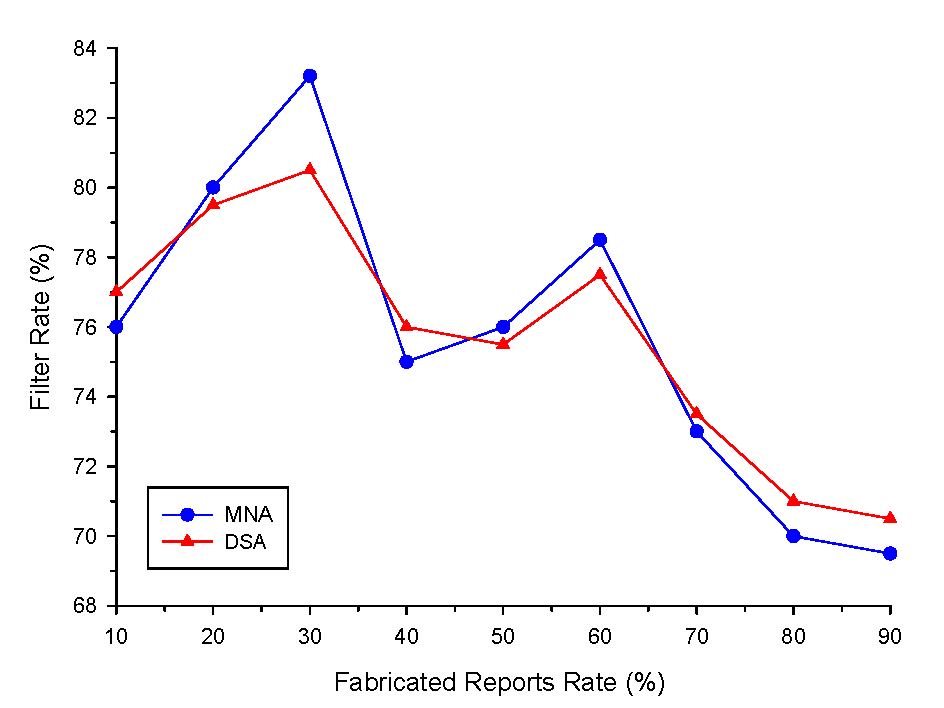
\includegraphics[width=5in]{DSAfilter}
  \caption{动态步长数据认证机制的安全性能}
  \label{fig:DSAfilter}
\end{figure}

如图~\ref{fig:DSAenergy}所示,是动态步长数据认证机制的能量开销。DSA方案相对MNA方案有较大的能量开销优化,尤其在FRR较小时,优化幅度较大。但是在FRR较大时,由于基站对网络安全状况的判定较低,无法维持步长的调整,压缩数据报文大小,因而能量开销的优化效果不明显。
\begin{figure}[htbp]
  \centering
  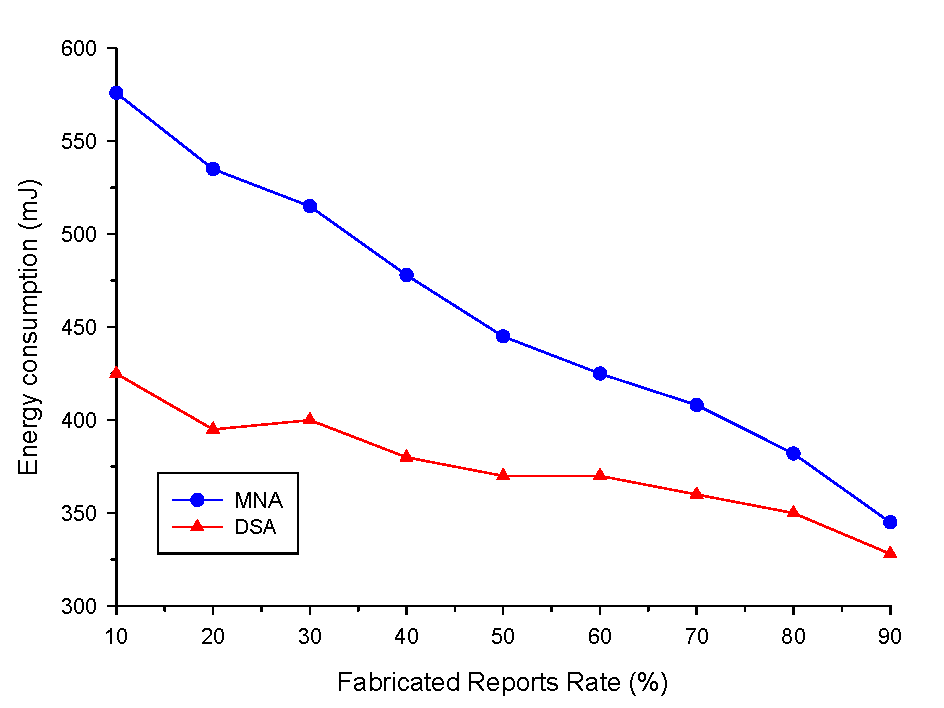
\includegraphics[width=5in]{DSAenergy}
  \caption{动态步长数据认证机制的能量开销}
  \label{fig:DSAenergy}
\end{figure}


\section{本章小结}
本章首先介绍了仿真实验环境的搭建,对使用OMNeT++进行无线传感网的仿真进行了介绍,对相关实验的框架搭建进行了说明。使用OMNeT++平台对我们的多跳长路径上多节点联合的数据认证机制进行仿真实验,验证该数据认证方案有较好的安全性能。
我们还对两个优化方案进行了仿真,实验结果表明两个方案分别对路径中检测率和通信开销有较好的改进。
